\documentclass{article}

\usepackage{graphicx}
\usepackage{tikz}
\usepackage{tikzsymbols}
\usetikzlibrary{calc,patterns,shapes.geometric}
\pagestyle{empty}
\usepackage[margin=0pt]{geometry}
\geometry{papersize={14in,12in}}

\def\centerarc[#1](#2)(#3:#4:#5){\draw[#1] ($(#2)+({#5*cos(#3)},{#5*sin(#3)})$) arc (#3:#4:#5);}

\begin{document}
	\begin{figure}
		\centering
		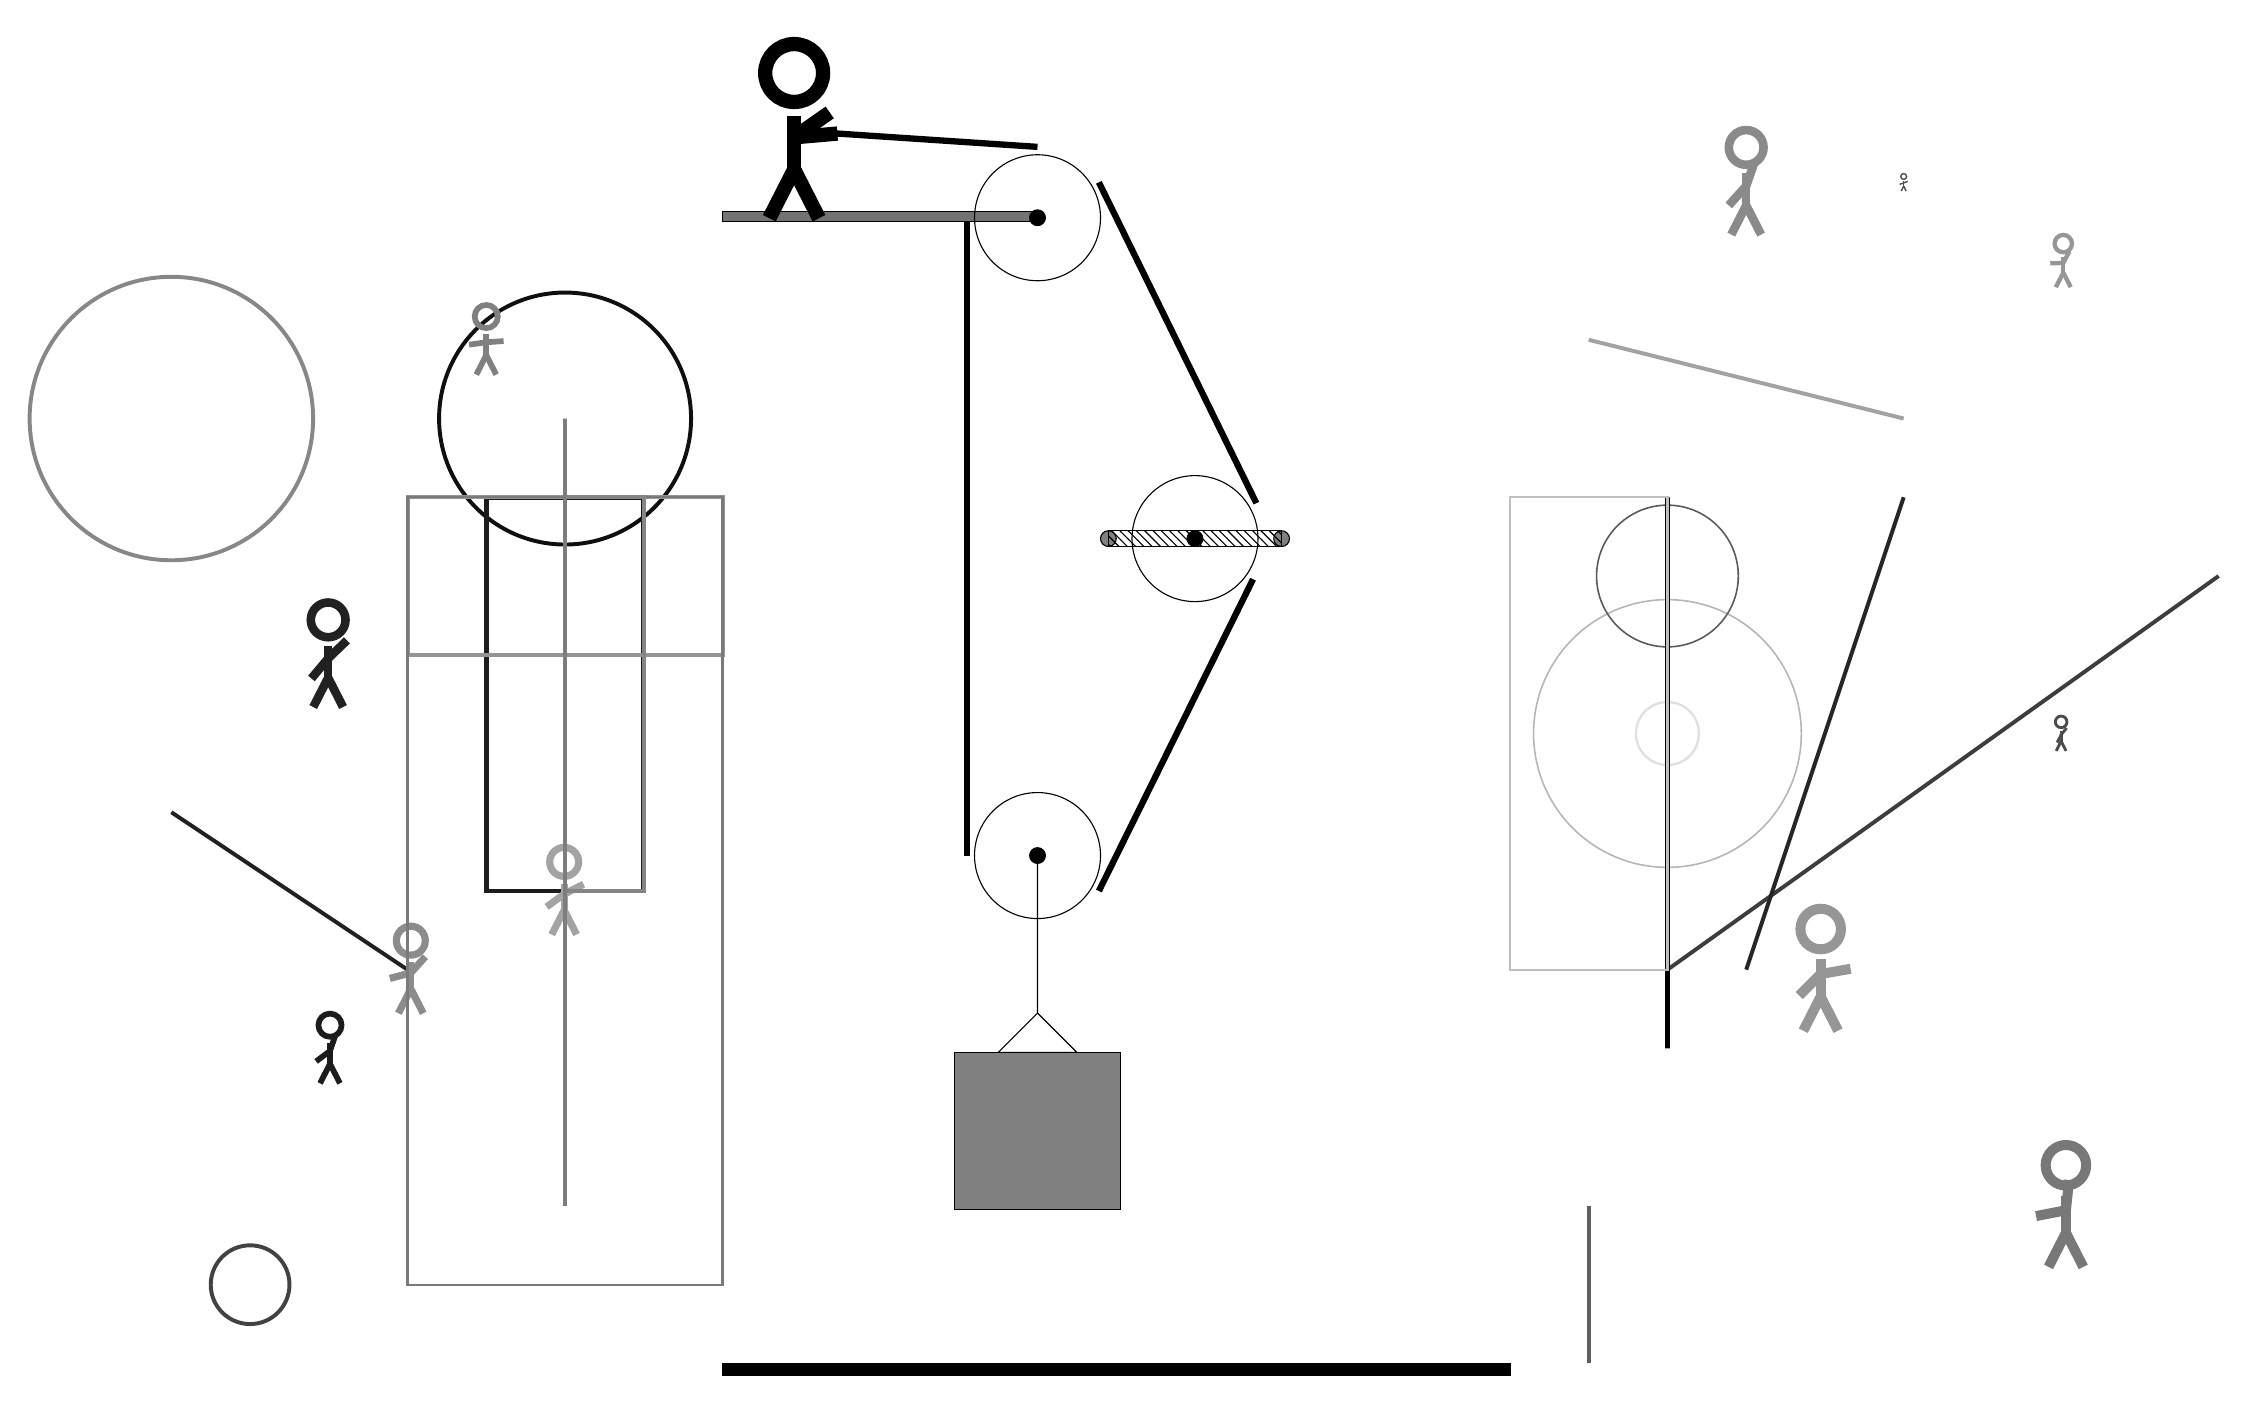
\begin{tikzpicture}
			%%%%% START %%%%%
			
			\draw[fill=black!55] (-2, 11.5) rectangle (2, 11.625);
			
			\draw (2, 3.45) circle (0.8);
			\draw[fill=black] (2, 3.45) circle (0.1);
			
			\draw (2, 11.55) circle (0.8);
			\draw[fill=black] (2, 11.55) circle (0.1);
			
			\draw[line width=0.5mm, color=black!37](9, 10) -- (13, 9);
			
			\draw[line width=0.5mm, color=black!87](-6, 2) -- (-9, 4);
			\draw [line width=0.5mm, color=black!94](-4, 9) circle (1.6);
			\draw[line width=0.5mm, color=black!63](9, -3) -- (9, -1);
			\draw[line width=0.5mm, color=black!76](10, 2) -- (17, 7);
			\node[line width=0.3mm, color=black!53] at (15, -1) {\Strichmaxerl[7][11][84]};
			\draw [line width=0.2mm, color=black!29](10, 5) circle (1.7);
			
			\draw [line width=0.2mm, color=black!65](10, 7) circle (0.9);
			\draw[line width=0.6mm, color=black!89] (-3, 3) rectangle (-5, 8);
			
			\draw [line width=0.3mm, color=black!12](10, 5) circle (0.4);
			\draw[line width=0.5mm, color=black!85](13, 8) -- (11, 2);
			\draw[line width=0.5mm, color=black!42] (-2, 8) rectangle (-6, 6);
			\draw [line width=0.5mm, color=black!74](-8, -2) circle (0.5);
			
			\node[line width=0.5mm, color=black!45] at (-6, 2) {\Strichmaxerl[5][15][48]};
			\node[line width=0.3mm, color=black!41] at (15, 11) {\Strichmaxerl[3][2][62]};
			\draw[line width=0.3mm, color=black!52] (-2, -2) rectangle (-6, 8);
			
			\node[line width=0.2mm, color=black!36] at (-4, 3) {\Strichmaxerl[5][36][27]};
			\node[line width=0.2mm, color=black!89] at (-7, 1) {\Strichmaxerl[4][37][71]};
			\node[line width=0.4mm, color=black!46] at (11, 12) {\Strichmaxerl[6][48][71]};
			
			\node[line width=0.3mm, color=black!69] at (13, 12) {\Strichmaxerl[1][19][22]};
			\draw [line width=0.5mm, color=black!47](-9, 9) circle (1.8);
			\draw[line width=0.5mm, color=black!48] (-3, 3) rectangle (-4, 8);
			\node[line width=0.3mm, color=black!50] at (-5, 10) {\Strichmaxerl[4][8][4]};
			\draw[line width=0.6mm, color=black!51] (-4, 9) rectangle (-4, -1);
			\draw[line width=0.7mm, color=black!100] (10, 8) rectangle (10, 1);
			\node[line width=0.5mm, color=black!87] at (-7, 6) {\Strichmaxerl[6][50][44]};
			
			\draw[line width=0.3mm, color=black!25] (8, 2) rectangle (10, 8);
			\node[line width=0.4mm, color=black!41] at (12, 2) {\Strichmaxerl[7][45][10]};
			\node[line width=0.4mm, color=black!70] at (15, 5) {\Strichmaxerl[2][63][51]};
			
			\draw[fill=white](4, 7.475) circle (0.8);
			\draw[fill=black] (4, 7.475) circle (0.1);
			\draw[fill=black!50] (2.9, 7.475) circle (0.1);
			\draw[fill=black!50] (5.1, 7.475) circle (0.1);
			\draw[pattern=north west lines, pattern color=black] (2.9, 7.575) rectangle (5.1, 7.375);
			
			\draw (2, 3.45) -- (2, 1.45) -- (1.5, 0.95) -- (2.5, 0.95) -- (2, 1.45);
			\draw[fill=black!50] (0.95, 0.95) rectangle (3.05, -1.05);
			
			\draw[line width=0.8mm] (1.1, 11.5) -- (1.1, 3.45);
			\centerarc[line width=0.8mm](2, 3.45)(180:330:0.9);
			\draw[line width=0.8mm](2.7794, 3.0) -- (4.7373, 6.9588);
			\centerarc[line width=0.8mm](4, 7.475)(390:325:0.9);
			\draw[line width=0.8mm](4.7794, 7.925) -- (2.7794, 12.0);
			\centerarc[line width=0.8mm](2, 11.55)(30:90:0.9);
			\draw[line width=0.8mm](2, 12.45) -- (-1, 12.65);
			
			\node at (-1, 12.65) {\Strichmaxerl[10][-175][35]};
			
			\draw[fill=black] (-2, -3) rectangle (8, -3.15);
			
			%%%%% END %%%%%
		\end{tikzpicture}
	\end{figure}	
\end{document}